\documentclass[11pt]{article}

\usepackage[french]{babel}
\usepackage[utf8]{inputenc}
\usepackage{tikz}
\usepackage{pgf}
\usetikzlibrary{arrows,automata}
\usepackage[left=2cm, right=2cm]{geometry}
\usepackage{amsmath}
\usepackage{listings}
\usepackage{graphicx}
\usepackage{multirow}

\date{}
\begin{document}

\def \ETScourse {ELE778-01 - Intelligence artificielle: réseaux neuroniques
et systèmes experts}
\def \ETStitle {Laboratoire 2}
\def \ETSprof  {Cynthia \textsc{Moussa}}
\def \ETSauthA {Liam \textsc{Beguin}\\\emph{BEGL02129304}}
\def \ETSauthB {Louis \textsc{Laporte}\\\emph{LAPL14128903}}
% Author : liambeguin
%
% To use this page add the following in your main page:
%
%\def \ETScourse {ELE430-01 - Conception des filtres Analogiques}
%\def \ETStitle {Laboratoire 2}
%\def \ETSprof {François \textsc{Gourlay}}
%\def \ETSauthA {Liam \textsc{Beguin}\\\emph{BEGL02129304}}
%\def \ETSauthB {Olivier \textsc{Belisle}\\\emph{BELO21098902}}
%\def \ETSauthC {bar}
%% Author : liambeguin
%
% To use this page add the following in your main page:
%
%\def \ETScourse {ELE430-01 - Conception des filtres Analogiques}
%\def \ETStitle {Laboratoire 2}
%\def \ETSprof {François \textsc{Gourlay}}
%\def \ETSauthA {Liam \textsc{Beguin}\\\emph{BEGL02129304}}
%\def \ETSauthB {Olivier \textsc{Belisle}\\\emph{BELO21098902}}
%\def \ETSauthC {bar}
%% Author : liambeguin
%
% To use this page add the following in your main page:
%
%\def \ETScourse {ELE430-01 - Conception des filtres Analogiques}
%\def \ETStitle {Laboratoire 2}
%\def \ETSprof {François \textsc{Gourlay}}
%\def \ETSauthA {Liam \textsc{Beguin}\\\emph{BEGL02129304}}
%\def \ETSauthB {Olivier \textsc{Belisle}\\\emph{BELO21098902}}
%\def \ETSauthC {bar}
%\input{titlepage.tex}

\newcommand{\HRule}{\rule{\linewidth}{0.5mm}}

\begin{titlepage}
	\begin{center}
		\vspace{5cm}
		\textsc{\textbf{\Huge \ETScourse}}
		\vspace{2cm}

		\textsc{\Large \ETStitle }
		\vspace{2.5cm}

		\textsc{\Large Pr\'esent\'e \`a : \\
		\ETSprof}
		\vspace{1.5cm}

		% Bottom of the page
		\vfill
		% Authors
		\begin{minipage}{0.4\textwidth}
			\begin{flushleft}
				\large\ETSauthA
			\end{flushleft}
		\end{minipage}
		\begin{minipage}{0.4\textwidth}
			\begin{flushright}
				\large\ETSauthB
			\end{flushright}
		\end{minipage}
		\begin{minipage}{0.4\textwidth}
			\begin{center}
				\large \ETSauthC
			\end{center}
		\end{minipage}

		\vspace{2cm}
		\HRule \\[0.4cm]
		{ \huge \bfseries \'Ecole de technologie superieure \\[0.4cm] }
		\HRule \\[1.5cm]
		\vspace{1.5cm}

		%date
		{\large \today}
	\end{center}
\end{titlepage}


\newcommand{\HRule}{\rule{\linewidth}{0.5mm}}

\begin{titlepage}
	\begin{center}
		\vspace{5cm}
		\textsc{\textbf{\Huge \ETScourse}}
		\vspace{2cm}

		\textsc{\Large \ETStitle }
		\vspace{2.5cm}

		\textsc{\Large Pr\'esent\'e \`a : \\
		\ETSprof}
		\vspace{1.5cm}

		% Bottom of the page
		\vfill
		% Authors
		\begin{minipage}{0.4\textwidth}
			\begin{flushleft}
				\large\ETSauthA
			\end{flushleft}
		\end{minipage}
		\begin{minipage}{0.4\textwidth}
			\begin{flushright}
				\large\ETSauthB
			\end{flushright}
		\end{minipage}
		\begin{minipage}{0.4\textwidth}
			\begin{center}
				\large \ETSauthC
			\end{center}
		\end{minipage}

		\vspace{2cm}
		\HRule \\[0.4cm]
		{ \huge \bfseries \'Ecole de technologie superieure \\[0.4cm] }
		\HRule \\[1.5cm]
		\vspace{1.5cm}

		%date
		{\large \today}
	\end{center}
\end{titlepage}


\newcommand{\HRule}{\rule{\linewidth}{0.5mm}}

\begin{titlepage}
	\begin{center}
		\vspace{5cm}
		\textsc{\textbf{\Huge \ETScourse}}
		\vspace{2cm}

		\textsc{\Large \ETStitle }
		\vspace{2.5cm}

		\textsc{\Large Pr\'esent\'e \`a : \\
		\ETSprof}
		\vspace{1.5cm}

		% Bottom of the page
		\vfill
		% Authors
		\begin{minipage}{0.4\textwidth}
			\begin{flushleft}
				\large\ETSauthA
			\end{flushleft}
		\end{minipage}
		\begin{minipage}{0.4\textwidth}
			\begin{flushright}
				\large\ETSauthB
			\end{flushright}
		\end{minipage}
		\begin{minipage}{0.4\textwidth}
			\begin{center}
				\large \ETSauthC
			\end{center}
		\end{minipage}

		\vspace{2cm}
		\HRule \\[0.4cm]
		{ \huge \bfseries \'Ecole de technologie superieure \\[0.4cm] }
		\HRule \\[1.5cm]
		\vspace{1.5cm}

		%date
		{\large \today}
	\end{center}
\end{titlepage}


\section{Introduction}
Après avoir fait une étape de pré-traitement lors du laboratoire 2.1, nous
allons maintenant implémenter un reseau de neurones a retro-propagation du
gradient d’erreur dans le but de classifier, le plus précisément possible,
le dataset TiDigits (english spoken digits from 1 to 9).

Pour implémenter ce reseau de neurones, nous utiliserons Python.
Voici une liste d'avantages versus inconvenients qui ont motive notre choix:
\begin{itemize*}
\item avantages:
	\subitem rapidite de developpement
		\subitem lang interprete, pas de compilation
		\subitem modules de calcul matriciel performants
		\subitem language accessible
	\item{inconvenients}
		\subitem lang interprete donc moins rapide \\
\end{itemize*}

Dans un premier temps, nous entrainerons le reseau sur un set de donnees puis
nous evaluerons sa capacite a generaliser sur de nouvelles donnees non utilisees
lors de l'entrainement.

\section{Implementation du r\'eseau de neurones}
\subsection{Architecture globale}
Etant donne que le reseau doit etre tres flexible quant au nombre de couches
et au nombre de neurones, nous utiliserons un tuple pour instancier
notre reseau. Chaque element de la liste represente une couche du reseau
(la couche d'entree etant compt\'ee) et sa valeur determine le nombre de neurones
present sur la couche.

\subsection{Extraction des donn\'ees}
% preprocessing, chx du 40, 50 ,60
% normalisation du dataset

\subsection{Initialisation du res\'eau}
Lorsque le reseau est instanci\'e, les parametres tels que $\eta$ et $\lambda$
sont copi\'es dans l'object
\emph{Network} et les matrices de poids et de seuils (\emph{weights} et
\emph{biases}) sont g\'en\'er\'ees. Les dimensions de ces matrices sont
determin\'ees en fonction du nombre de neurones sur chaque couche et du nombre
de couches $L$ \`a l'aide de la methode suivante:

Soit, $w_{ij}^{(l)}$ le poid connectant le neurone $i$ de la couche $(l-1)$ au
neurone $j$ de la couche $(l)$. \\
O\`u :
\begin{equation}
	\left \{
	\begin{aligned}
		&1 \le l \le L \\
		&0 \le i \le d^{(l-1)} \\
		&1 \le j \le d^{(l)} \\
	\end{aligned}
	\right .
\end{equation}
On definit donc ${\bf w}^{(l)}$ la matrice de dimension $((l) \times (l-1))$
connectant la couche $(l-1)$ \`a la couche $(l)$ cr\'eant ainsi, $(L-1)$ matrices
de poids sur l'ensemble du reseau. \\

D'autre part, du fait que la fonction aleatoire utilis\'ee pour l'initialisation
des poids donne une distribution avec les parametres suivants $\mu=0$ et $\sigma=1$,
l'initialisation des poids a tendance a saturer les neurones et ralentire l'apprentissage.
car :
\begin{equation}
	\begin{aligned}
		Var(z) &= \sum_{i=1}^N(Var(x_i)) \\
		Var(z) &= N \cdot Var(x) \\
		\sigma(z) &= \sqrt{N} \cdot 1 \\
		\sigma(z) &= \sqrt{N}
	\end{aligned}
\end{equation}




\begin{figure}[htp]
	\centering
	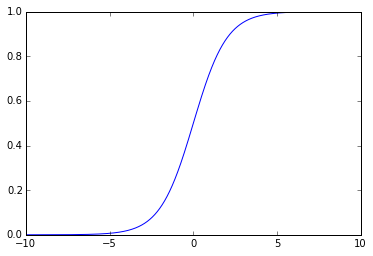
\includegraphics[scale=.5]{img/sigmoid_sat.png}
	\caption{Visualisation de la saturation de la fonction \emph{sigmoid} si
	$|z| \ge 5$.}
\end{figure} \\

Pour contrer cette saturation et donc accelerer les premi\`eres \'epoques
d'apprentissage, nous utiliserons une distribution plus \'etroite avec les
parametres $\mu=0$ et $\sigma =1/\sqrt{N}$ \\


\lstset{tabsize = 4,
frame=lines,
numbers=left,
captionpos=b,
caption = {Initialisation des poids et seuils},
language = python,
basicstyle=\small} \\
\begin{lstlisting}
self.biases  = [ np.random.randn(y, 1) for y in struct[1:] ]
self.weights = [ np.random.randn(y, x) / np.sqrt(x) \
				for x, y in zip(struct[:-1], struct[1:]) ]
\end{lstlisting}


\subsection{Fonctions d'activation}
% sigmoid  -> probability dist
% tanh     -> soft threshold (linear arround 0 hard threshold far)
% softplus -> linear above 0
% add plots



\subsection{Fonctions de cout}
% cross-entropy -> prevent neuron saturation

\subsection{Eviter le sur-apprentisage}
% plus ya de neurons plus on peut overfit -> polynome a plus de dimensions
\subsubsection{Early stopping}
% add this image https://upload.wikimedia.org/wikipedia/commons/thumb/1/1f/Overfitting_svg.svg/1024px-Overfitting_svg.svg.png?1469206069861
\subsubsection{Validation crois\'ee}
% leave one out, K folds, implique de 'bouger' des trucs dans les datasets
% merge train et VC -> larger traiing set
\subsubsection{Fonctions de r\'egularisation}
% penalise le poids large check :
% http://neuralnetworksanddeeplearning.com/chap3.html#overfitting_and_regularization

\subsection{Entrainement}
% batch gradient descent
% stochastic gradient descent
% minibatch GD check network.py

\subsection{Ajustement des hyper-param\`etres}
% http://neuralnetworksanddeeplearning.com/chap3.html#how_to_choose_a_neural_network's_hyper-parameters

\subsection{Inspection du res\'eau}

\section{Interface graphique}



\section{Discussions}
\subsection{Problemes rencontr\'es}
\subsection{Methodes de r\'esolution}
\subsection{conclusion et possibilites d'amelioration}
% ajouter autres pistes d'amelioration
% conclure sur performance globale du systeme
% classification homme/femme

\end{document}
% vim: cc=80 :
